\documentclass[letterpaper]{article}
\usepackage{natbib,alife13}

\title{Aracna: An Open-Source Quadruped Platform for Evolutionary Robotics}
\author{Sara Lohmann, Eric Gold, Jeremy Blum, Jason Yosinski \and Hod Lipson \\
\mbox{}\\
Cornell University, 239 Upson Hall, Ithaca, NY 14853 \\
\texttt{sml253@cornell.edu}}



\begin{document}
\maketitle

\begin{abstract}
We report on a new open-source quadruped robotic platform, Aracna,
for evolutionary robotics experiments. The robot comprises four legs
with two joints each, for a total of eight kinematic degrees of
freedom. Four-bar linkage mechanisms in each leg drive the pitch of
the knee joint and the hip joint remotely, allowing the motors to
remain in the robot center, thereby reducing the inertia of each
leg. Due to these non-conventional kinematics, the robot requires non
intuitive movements for locomotion that are challenging for
learning. We suggest that this platform can provide a low-cost,
accessible platform for testing and comparing physical evolutionary
robotics algorithms.
\end{abstract}



\section{Introduction}

We address the need for a low-cost platform with non-intuitive walking
kinematics to explore evolutionary robotics. Aracna is the third
evolutionary learning quadruped robot developed by the Creative
Machines Lab \citep{HL, JY}. A common feature among the quadruped
robots is two actuators that drive the flexion/extension of a knee and
hip joint around parallel axes in each leg. The original Creative
Machines Lab quadruped robot favored starfish-like movements
\citep{HL}. The second quadruped robot, QuadraTot \citep{JY},
developed spider-like movements, but was limited by its weight. When
creating the Aracna, we designed the hardware to compliment fast
spider-like movements.

\begin{figure}[t]
\begin{center}
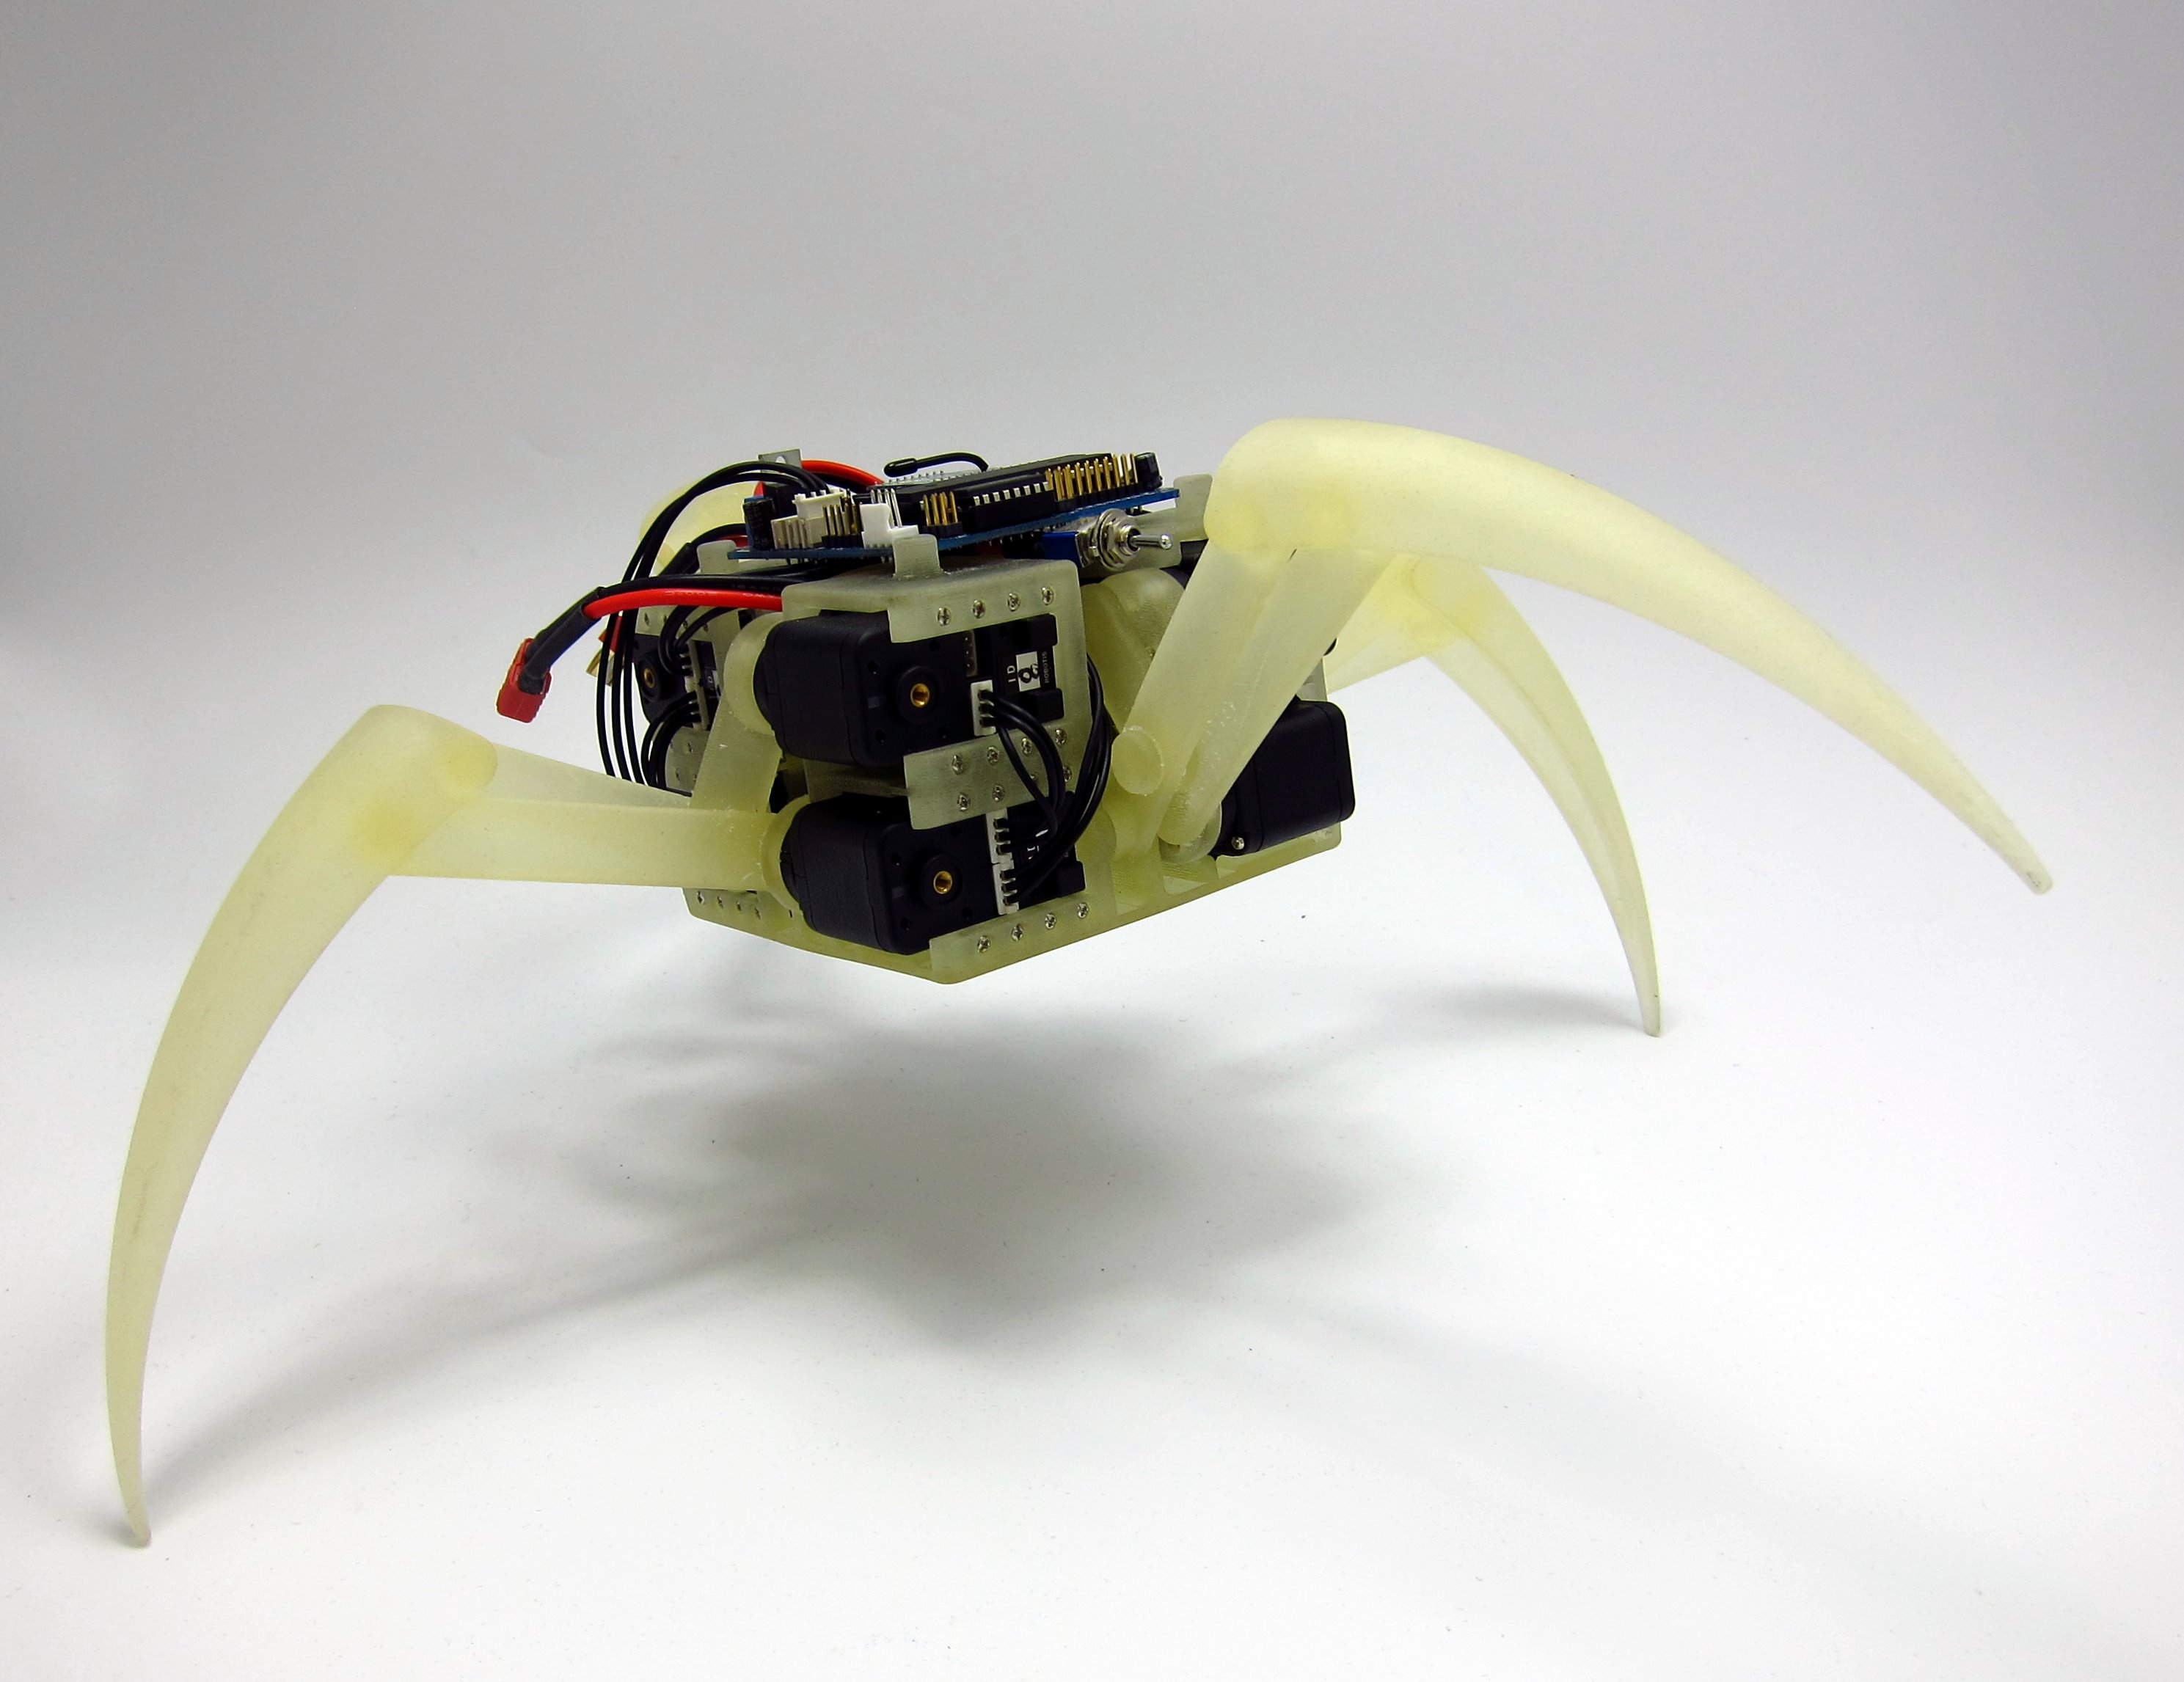
\includegraphics[width=.45\textwidth]{fig1.jpg}
\caption{Aracna: an open-sourced quadruped robot platform. All
  instructions and downloads are publicly available at
  http://creativemachines.cornell.edu/quadrarex \citep{WEB}.}
\label{fig1}
\end{center}
\end{figure}



\section{Hardware}

\begin{figure}[t]
\begin{center}
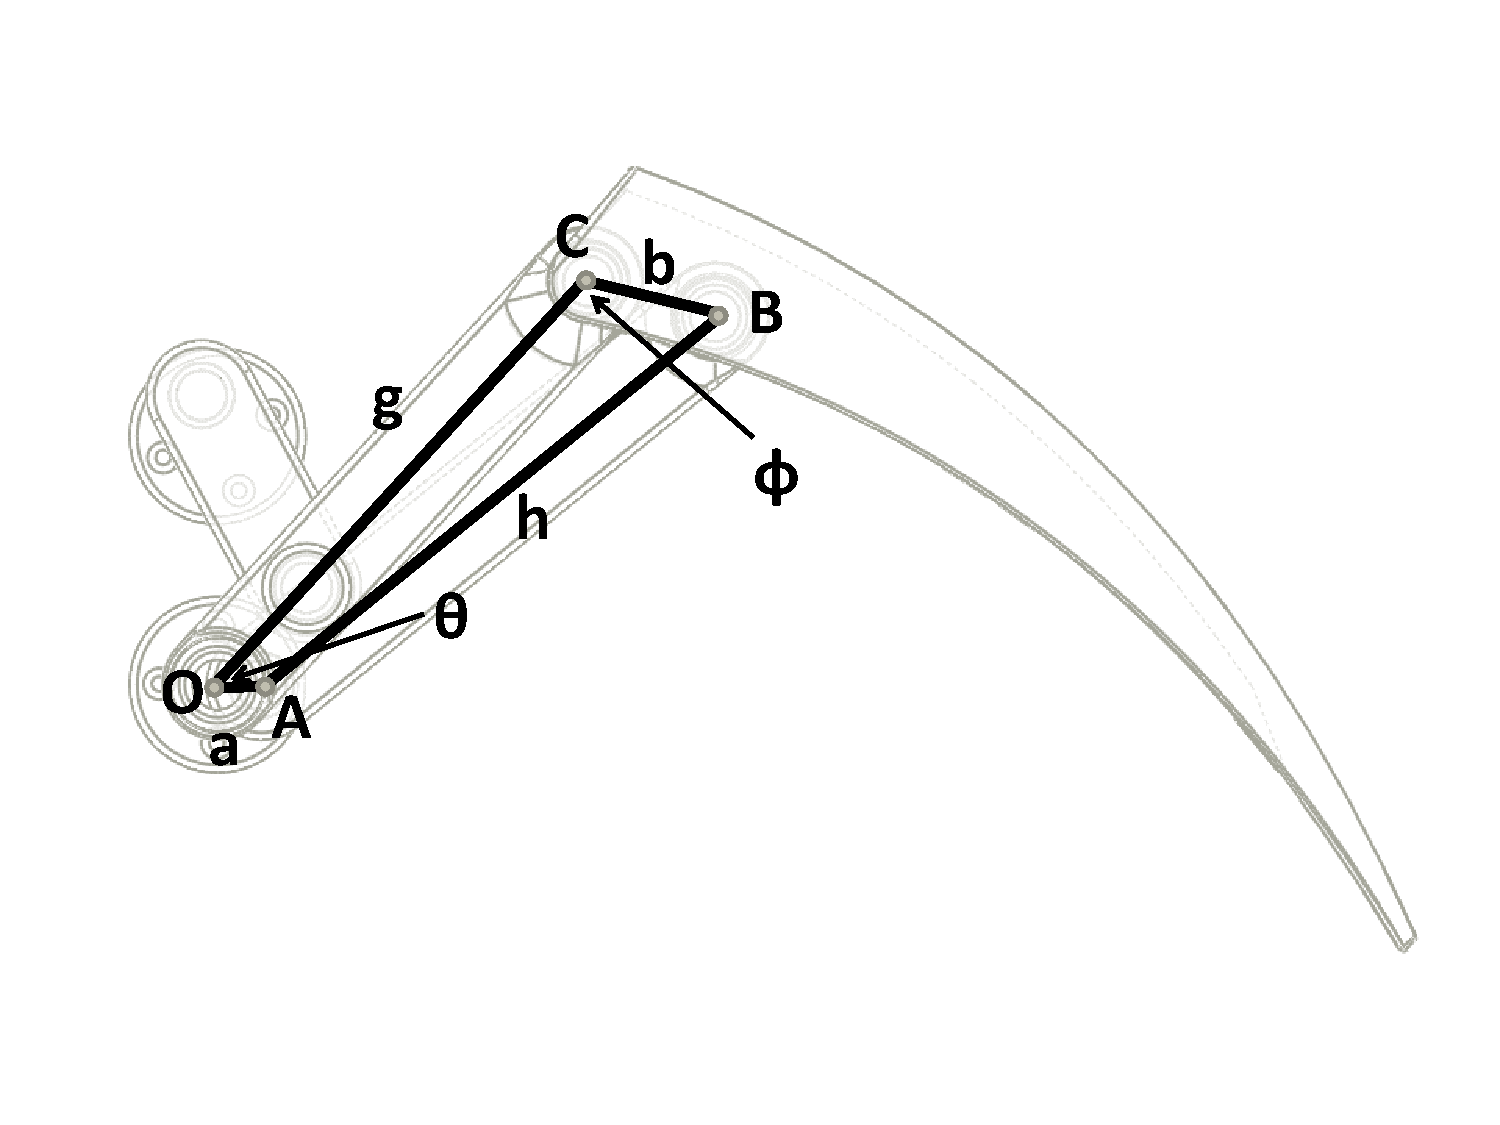
\includegraphics[width=.23\textwidth]{fig3.pdf}
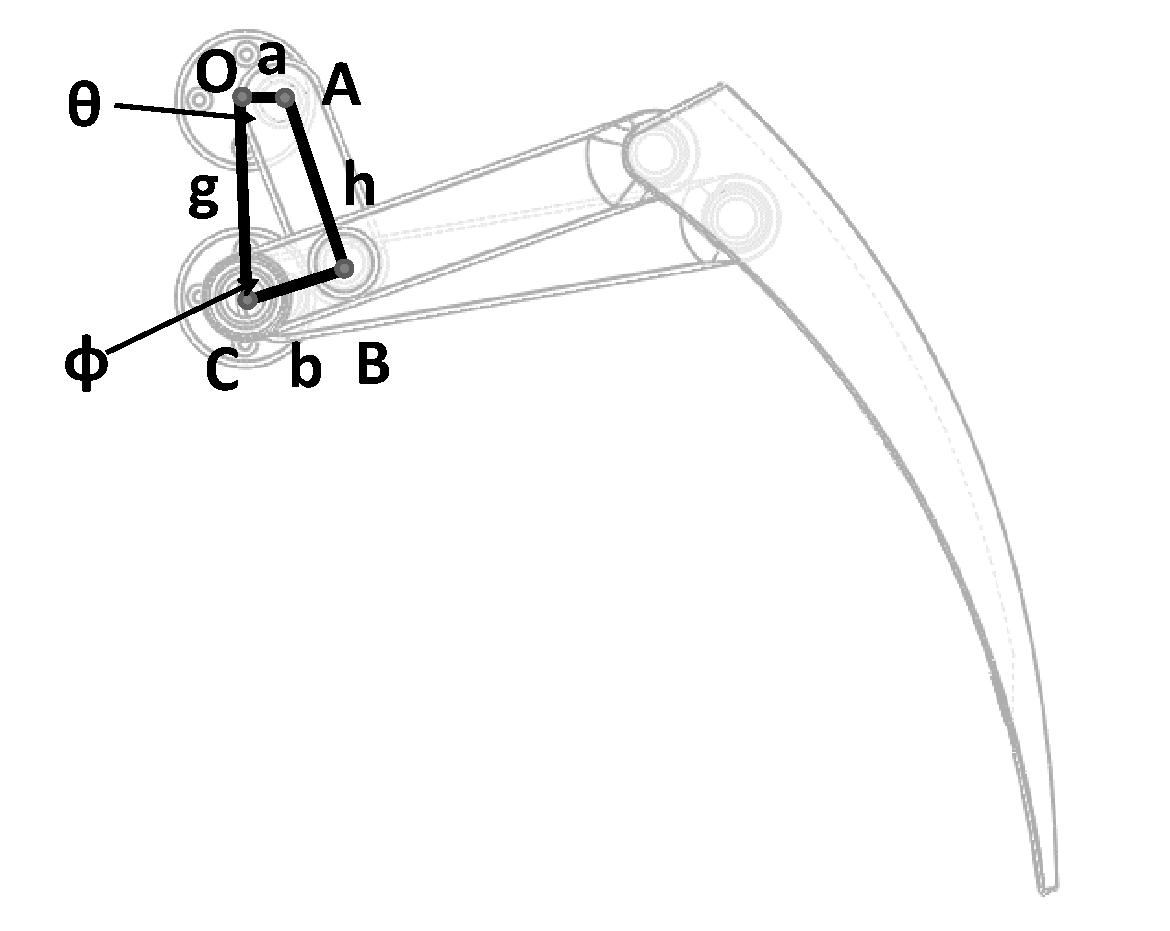
\includegraphics[width=.23\textwidth]{fig4.pdf}
\caption{Crank-rocker 4 bar linkage controlling flexion/extension of
  the knee and hip joints.}
\label{fig3}
\end{center}
\end{figure}

%\begin{figure}[t]
%\begin{center}
%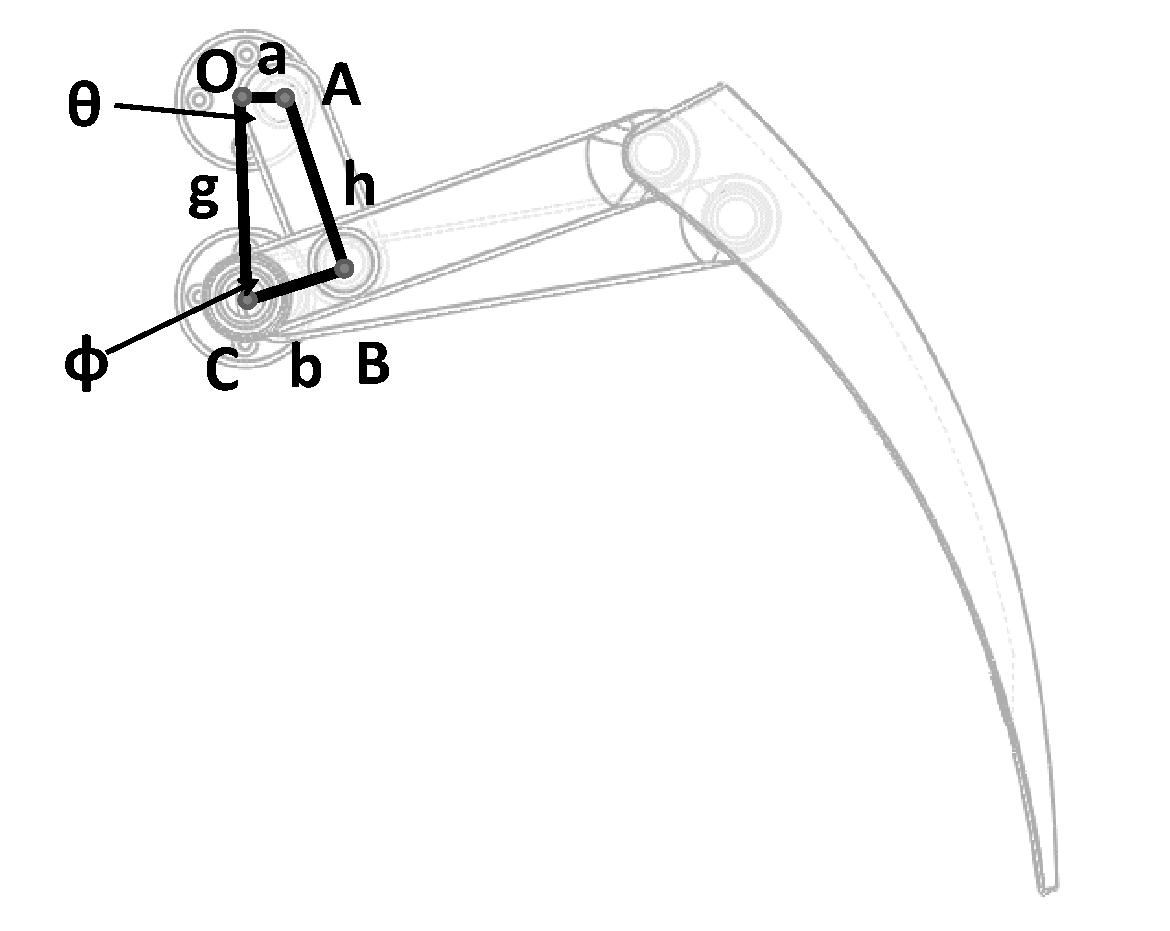
\includegraphics[width=2.25in,angle=0]{fig4.pdf}
%\caption{Crank-rocker 4 bar linkage controlling flexion/extension of the hip joint.}
%\label{fig4}
%\end{center}
%\end{figure}

The hardware of Aracna evolved from the previous Creative Machines
Lab quadruped robots. We kept the same two degree of freedom pitch
joint scheme but decreased the weight and constrained the movement of
the joints to create faster spider-like movement. To prevent
starfish-like movement, the legs were constrained. We designed the
robot with two four bar mechanisms to drive the joints in each
leg. With a four bar mechanism in place, the leg moves at a fraction
of the output angle of the actuator. Figure~\ref{fig3} shows the
crank-rocker system, where the input crank (link OA) is actuated by a
servo, the rocker is the leg (link CB), and the fixed link is OC. In
this configuration, we keep the servo motors contained in the center
of the robot, thereby reducing the inertia of each leg. The four bar
mechanisms satisfied the design goal of making a robot that had
non-traditional movements. We avoided designing a robot similar to an
off-the-shelf robot to create something unique. To make the robot
accessible as an open-source platform, it was designed to be 3D
printed. The 3D print files and CAD files can be accessed by the
public to be modified and printed.  \\ We designed the robot to be
lightweight to focus on the goal of evolutionary robotics. We use a
single LiPo 11.1V battery to power 8 Dynamixel AX-18 servo motors and
an ArbotiX microcontroller. The main processing occurs on an external
computer, which allows the robot to have cheaper and lighter
components on-board. We use the space in the center of the body to
house the battery to reduce material weight and cost. Aracna weighs
less than 1 kg.

\begin{figure}[t]
\begin{center}
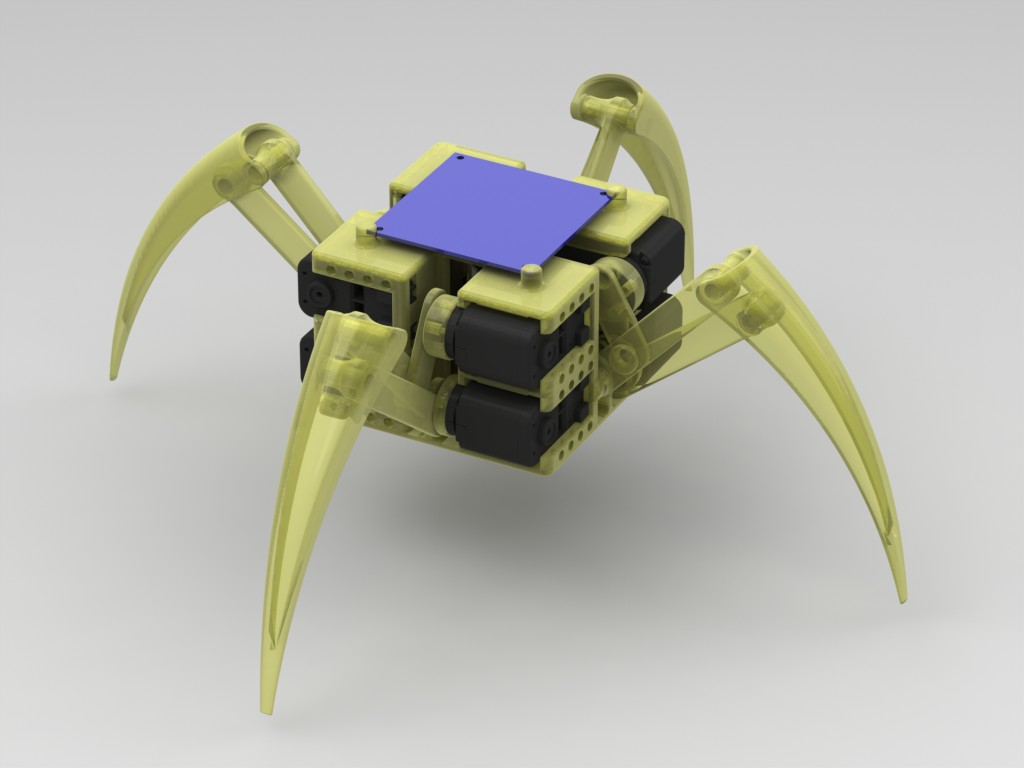
\includegraphics[width=2.25in,angle=0]{fig5.jpg}
\caption{Renderd CAD model.}
\label{fi52}
\end{center}
\end{figure}



\section{Software}

The software is open-sourced code written in Python based on the
evolutionary learning algorithms of the QuadraTot \citep{JY}. We
provide the controller code on our website \citep{WEB}. We use an
external computer for processing. We use an infrared light emitting
diode on the robot along with an external Wii remote to provide
feedback of the distance traveled. The external computer receives
feedback from the Wii remote and internal servo sensors and then
processes the information to send the next command to position the
servos. The communication between the external computer and the
ArbotiX on-board microcontroller occurs over wireless XBee.



\section{Specifications}

\begin{figure}[t]
\begin{center}
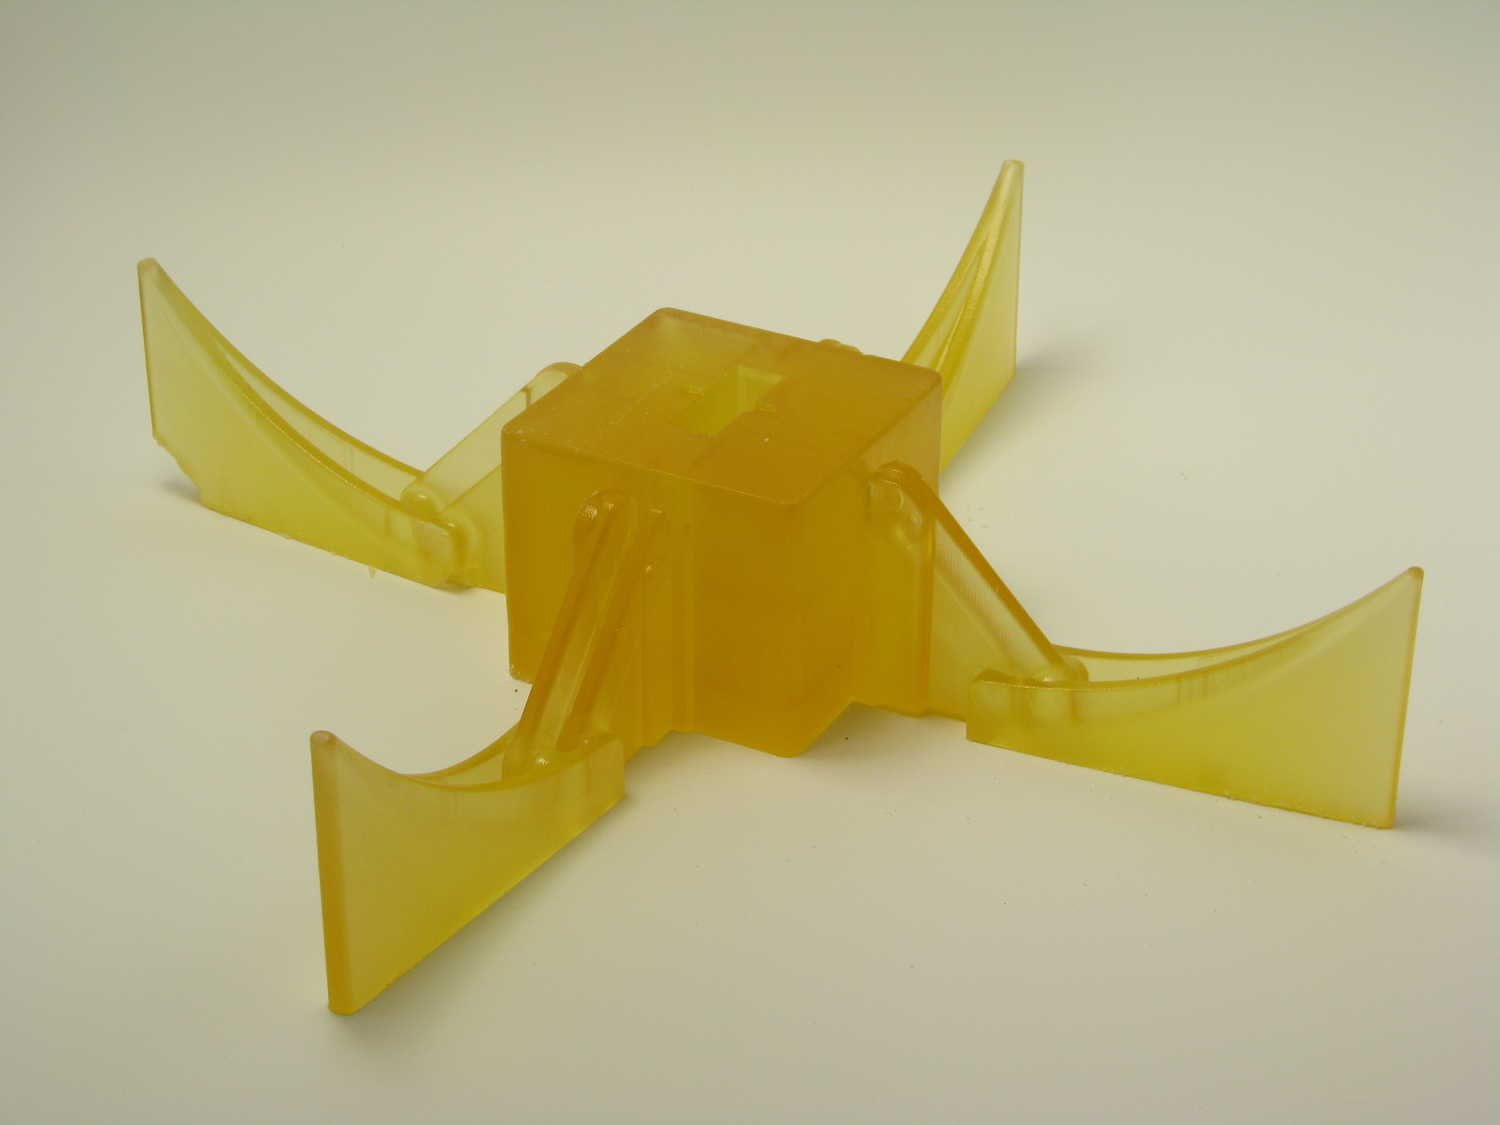
\includegraphics[width=2.25in,angle=0]{fig2.jpg}
\caption{Robot printed as one piece with support material intact.}
\label{fig2}
\end{center}
\end{figure}

We 3D printed the robot as one part (Figure~\ref{fig2}). The robot was
completed after approximately 26 hours, and used approximately 1000 g
of model material and 1500 g of support material. We estimated the
cost of the printed parts to be \$410 by using the estimated model
material cost to be \$1/4.5g and the support material cost to be
\$1/8g. This cost estimate is highly variable depending on the type of
material used. The robot has no removable printed parts except for the
battery cover. We will make the robot available to print as separate
parts for smaller 3D printer tray sizes. Printing the robot as
separate parts will reduce the amount of support material and cost to
print. We estimated the total cost to be less than \$1500 for the
custom robot platform. We made these estimates based on the material
calculations above and prices from trossenrobotics.com.

\begin{table}[h]
\center{
\begin{tabular}{|c|c|}
\hline
Part & Cost\\
\hline\hline
3D Print Materials & \$410.00\\
ArbotiX Robocontroller Kit & \$189.00\\
Dynamixel AX-18A Robot Actuator (x8) & \$721.28\\
3S 11.1V 2000mAh Pro Lite LiPo Battery & \$72.99\\
LiPo Battery Balance Charger Kit & \$69.99\\
Cables, Connectors, Misc & \$27.78\\
\hline\hline
\bf Total & \bf \$1491.04\\
 \hline
\end{tabular}
}
\vskip 0.25cm
\caption{Estimated total cost. A specific parts list is on our website \citep{WEB}.}
\end{table}



\section{Acknowledgements}

This work was supported by the National Science Foundation's Office of
Emerging Frontiers in Research and Innovation (grant number 0735953).


\footnotesize
\bibliographystyle{apalike}
\bibliography{references}
\end{document}

